%% Overleaf			
%% Software Manual and Technical Document Template	
%% 									
%% This provides an example of a software manual created in Overleaf.

\documentclass{ol-softwaremanual}

% Packages used in this example
\usepackage{graphicx}  % for including images
\usepackage{microtype} % for typographical enhancements
% \usepackage{minted}    % for code listings
\usepackage{amsmath}   % for equations and mathematics
% \setminted{style=friendly,fontsize=\small}
% \renewcommand{\listoflistingscaption}{List of Code Listings}
\usepackage{hyperref}  % for hyperlinks
\usepackage[a4paper,top=4.2cm,bottom=4.2cm,left=3.5cm,right=3.5cm]{geometry}
\usepackage{authblk}
\usepackage{pdfsync}
\usepackage{boldline}
\usepackage{longtable}
\usepackage[version=3]{acro}
\usepackage{gensymb}
% \usepackage[printonlyused,withpage]{acronym}
\usepackage[numbers,sort&compress]{natbib}
\usepackage{anysize}
% \marginsize{2cm}{2cm}{1.cm}{1.cm}
\usepackage{graphicx}
\usepackage{epsfig}
\usepackage{verbatim} 
\usepackage{bm}
\usepackage{etoolbox}
%\usepackage{amssymb}
%\usepackage{amsfonts,amsmath}
\usepackage{multirow}
% \usepackage[T1]{fontenc}
\usepackage{yfonts}
\usepackage{xr-hyper} 
% \externaldocument{manuscript}
\usepackage{xcite} 
% \externalcitedocument{manuscript}
\usepackage{mathrsfs}
% \usepackage{fancyhdr}
% \usepackage{relsize}
%  \usepackage{newpxtext,newpxmath}
%  \usepackage{booktabs,siunitx}
\usepackage{array,booktabs,ragged2e}
\usepackage{enumitem}   
\usepackage{empheq}
\usepackage[font=small,labelfont=bf]{caption}
\usepackage[title,toc,titletoc,page]{appendix}
\usepackage[capitalise]{cleveref}
\usepackage[most]{tcolorbox}
\usepackage{tocloft}
\usepackage{eurosym}
% \usepackage[colorlinks]{hyperref}

 % for setting page size and margins

% Custom macros used in this example document
\newcommand{\doclink}[2]{\href{#1}{#2}\footnote{\url{#1}}}
\newcommand{\cs}[1]{\texttt{\textbackslash #1}}

\acsetup{
  make-links ,
  pages / display = first ,
  pages / fill    = {, }
}

\hypersetup{colorlinks=true,
	linkcolor=blue,
	anchorcolor=black,
	citecolor=red,
	urlcolor=blue
}

\DeclareAcronym{UTC}{short = UTC, long = Universal Time Coordinated}
\DeclareAcronym{TAI}{short = TAI, long = International Atomic Time}
\DeclareAcronym{nm}{
    short = nm, 
    short-plural-form = {nm},
    long = nautical mile
    }
\DeclareAcronym{km}{
        short = km, 
        short-plural-form = {km},
        long = kilometer
}
\DeclareAcronym{hr}{
        short = h, 
        short-plural-form = {hrs},
        long = hour
}
\DeclareAcronym{min}{
        short = min, 
        short-plural-form = {mins},
        long = minute
}
\DeclareAcronym{sec}{
        short = s, 
        short-plural-form = {s},
        long = second
}
\DeclareAcronym{kt}{
    short = kt, 
    short-plural-form = {kts},
    long = knot
    }
\DeclareAcronym{ft}{
    short = ft, 
    short-plural-form = {ft},
    long = foot,
    long-plural-form = {feet}
    }
\DeclareAcronym{m}{
    short = m, 
    short-plural-form = {m},
    long = meter
    }

\DeclareAcronym{N}{
    short = N, 
    long = North
}
\DeclareAcronym{S}{
    short = N, 
    long = South
}
\DeclareAcronym{E}{
    short = E, 
    long = East
}
\DeclareAcronym{W}{
    short = W, 
    long = West
}
\providecommand{\thel}{Thelemacus\,\,}


% Frontmatter data; appears on title page
\title{Documentation}
\version{1.0}
\author{Michele Castellana}
\softwarelogo{\includegraphics[width=8cm]{logo}}

\begin{document}

\maketitle

\tableofcontents
% \listoflistings
\newpage

\section{Introduction}


\thel  is a navigational-astronomy application, which allows to compute one's position on the surface of the Earth, on both land and sea, based on sextant measurements. \thel is conceived to make the user's life easy, and it is designed for an intuitive and quick use. 

\subsection{Thelemacus is free software}

\thel is ``free software''; this means that everyone is free to use it. The software is not in the public domain \cite{castellana2024thelemacus}; it is copyrighted and there are conditions on its distribution. These conditions are designed to permit everything that a good cooperating citizen would want to do.

\subsection{Obtaining Thelemacus}

The source code for the library can be obtained from the GitHub repository \href{https://github.com/mcastel1/thelemacus}{mcastel1/thelemacus}. The executable can be downloaded from my \href{https://sites.google.com/site/michelecastellana/home}{website}, for OSx and Windows.  

Announcements of new releases, updates and other relevant events are made \href{https://sites.google.com/site/michelecastellana/home}{online}. 

\subsection{No warranty}

The \thel has no warranty, it is provided ``as is.'' It is your responsibility to validate the behavior of \thel and its accuracy using the source code provided, or to purchase support and warranties from commercial redistributors. Consult \thel's  License for further details.

\subsection{Reporting bugs}

A list of known bugs can be found in the \href{https://github.com/mcastel1/thelemacus/issues}{issues} section of the GitHub repository.
If you find a bug which is not listed in there, please report it to \href{mailto:michele.castellana@gmail.com}{me}. All bug reports should include:
\begin{itemize}
    \item The version number of \thel, 
    \item The hardware and operating system, 
    \item A short description of the bug behavior. 

\end{itemize}

Any errors or omissions in this manual can also be reported to the same address.


\subsection{Further information}


Additional information, including online copies of this manual, links to related projects, and mailing list archives are available from the \href{https://sites.google.com/site/michelecastellana/home}{website}  above.
Any questions about the use and installation of \thel can be asked by \href{mailto:michele.castellana@gmail.com}{email}. This mailing address can be used to ask questions not covered by this manual, and to contact the developers of the library.

If you would like to refer to \thel in a journal article, the recommended way is to cite this reference manual \cite{castellana2024thelemacus-documentation}. If you want to give a url, use  \href{https://sites.google.com/site/michelecastellana/home}{this one}. 



\section{Using \thel}

\subsection{The main frame}

\subsection{The sight frame: taking a sight}

In order to use \thel, the user needs to be familiar with taking a celestial sight with a sextant, please see \cite{bowditch2002the} for details. 

\begin{figure}
  \centering
  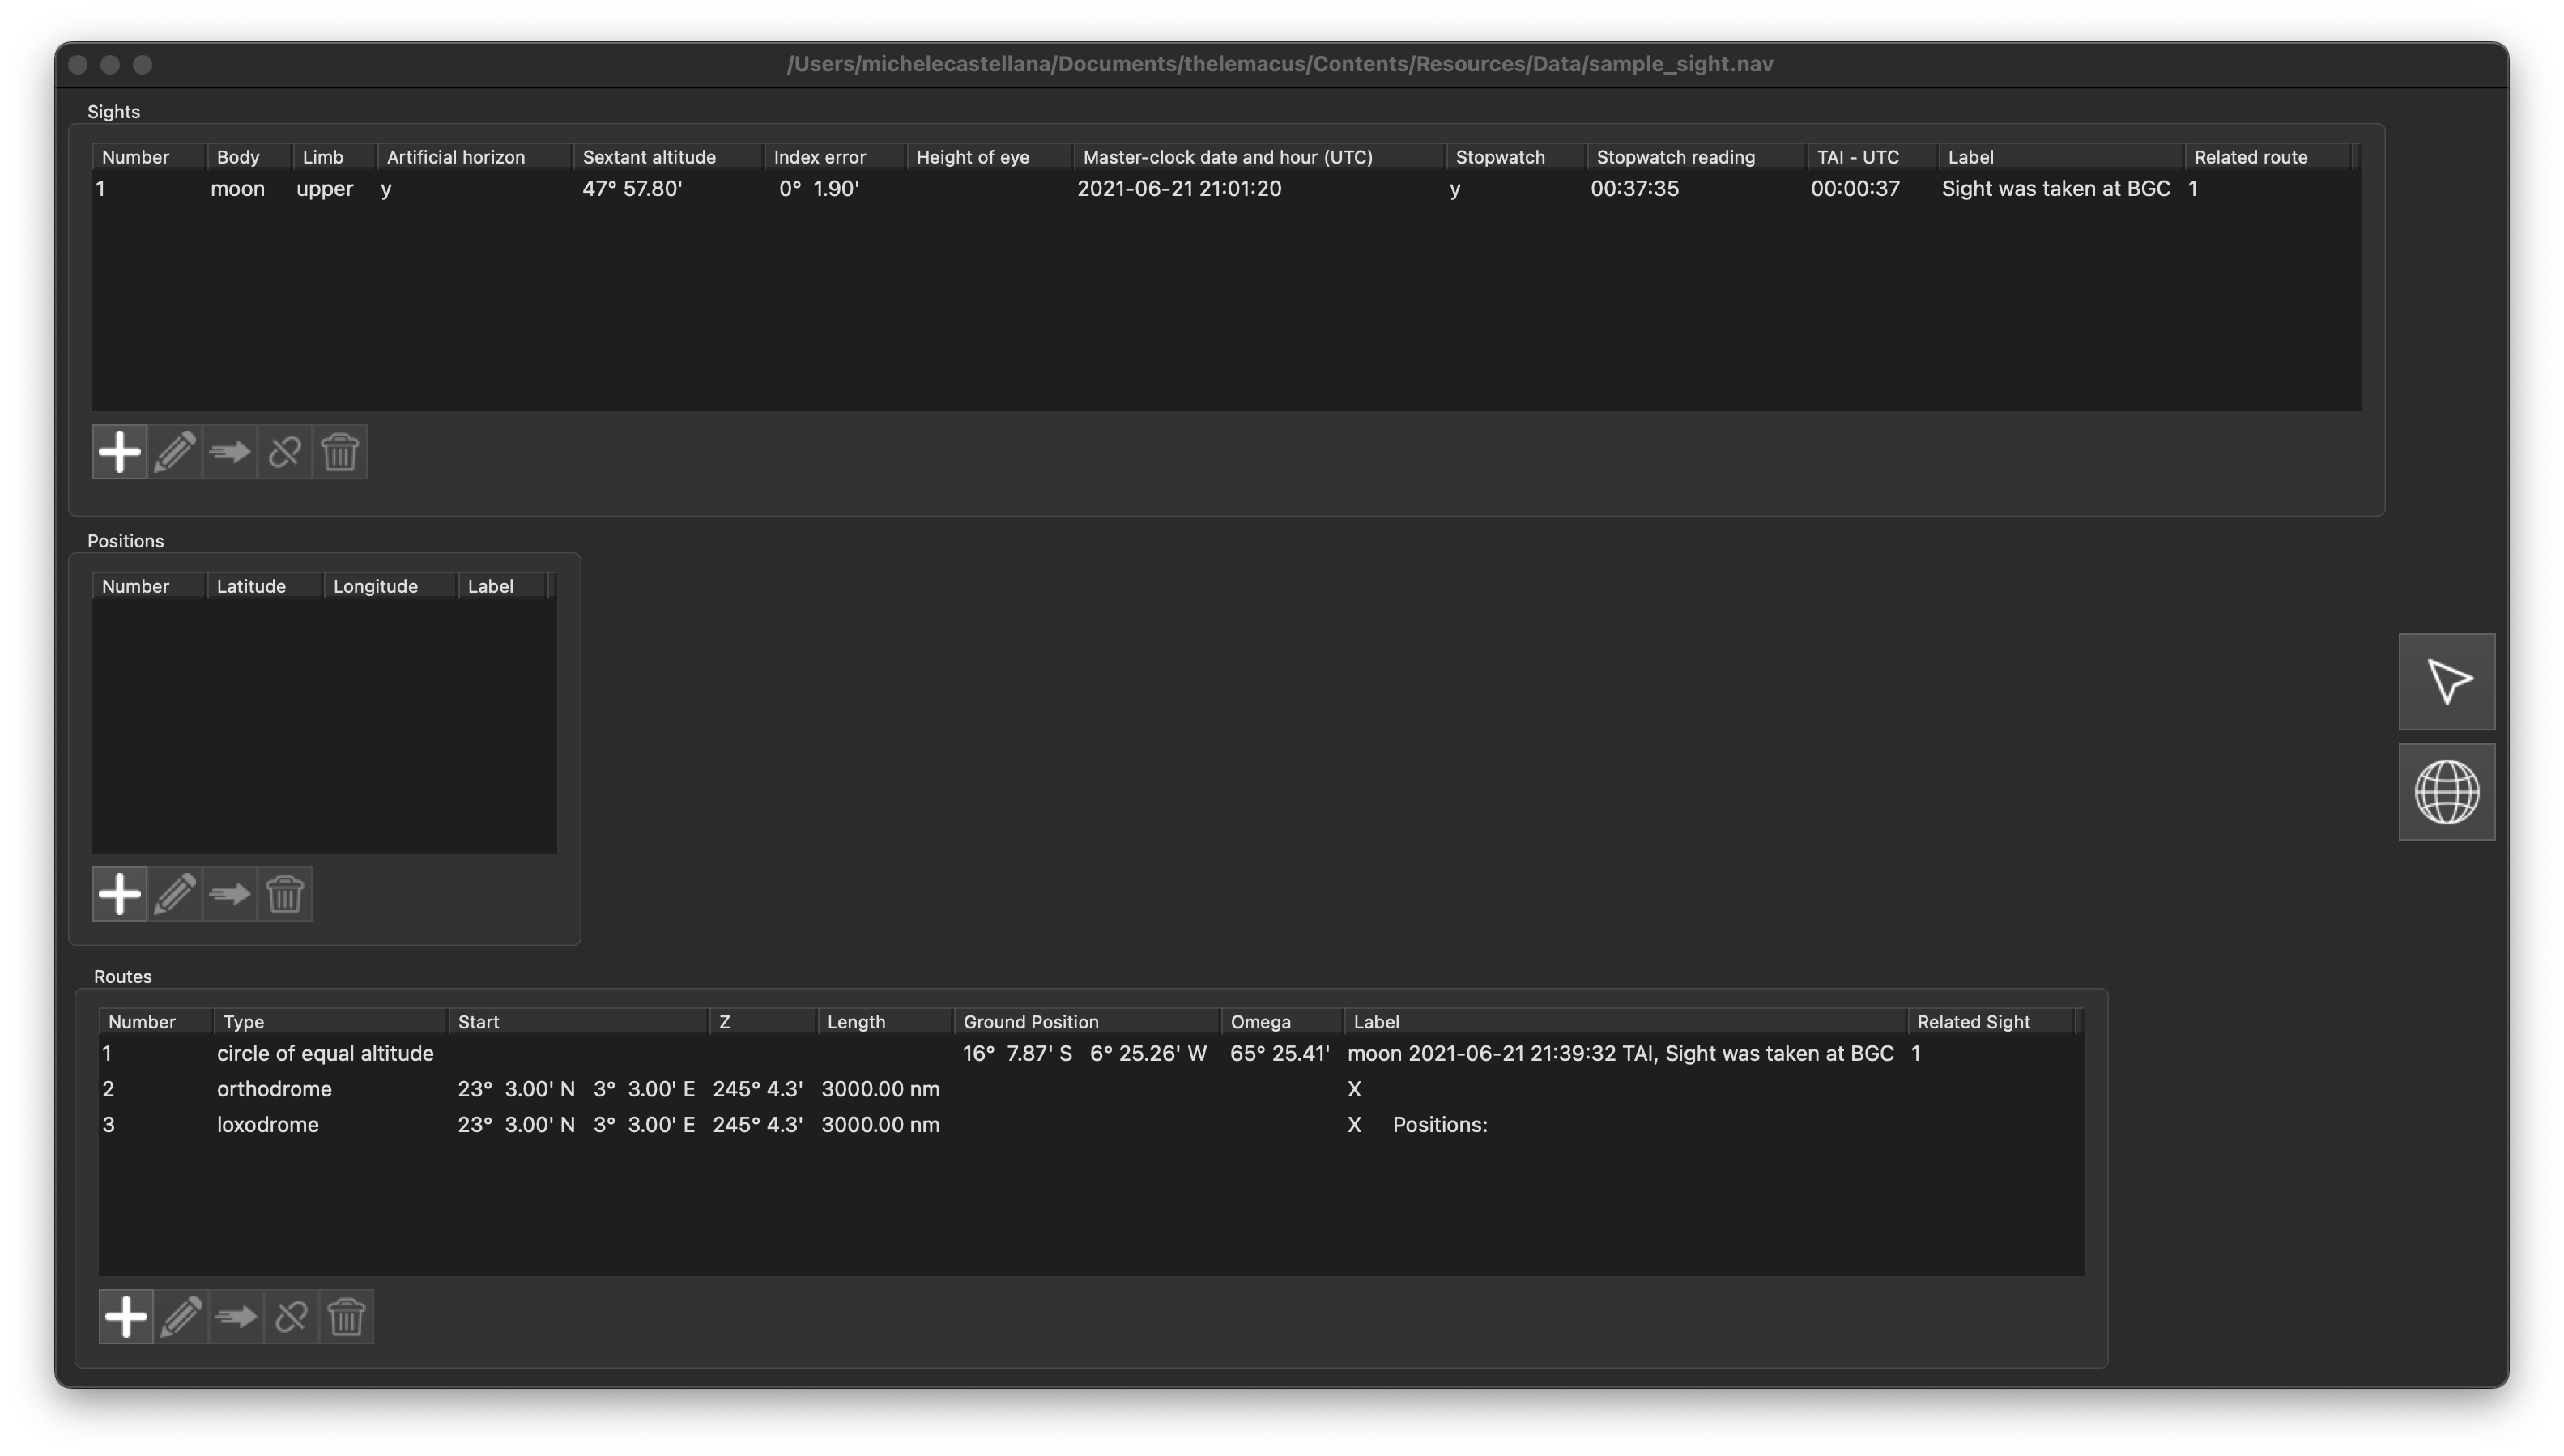
\includegraphics[width=1\textwidth]{figures/list-frame.png}
  \caption{
    \label{fig-list-frame}
    The main frame of \thel. 
  }
  \end{figure}

The results of this measurements will be 
\begin{enumerate}
\item \label{item-name} The name of the celestial body, e.g. the star `Arcturus'
\item \label{item-limb}  If the body is the Sun or the Moon, the limb (`upper', `center' or `lower') of the body which has been considered in the measurement
\item \label{item-body-height} The angular height of the celestial body over the horizon, expressed in degrees and arcminutes, e.g., $54 \degree \, 45.34'$
\item \label{item-artificial-horizon} Whether the observer used an artificial horizon or not
\item \label{item-time} \ac{UTC} date and time of the measurement, e.g., $2024$-$11$-$4$ $22$:$04$:$23$ \ac{UTC}
\item \label{item-label} A label for the sight (optional), e.g., `First sight of my night shift'
\end{enumerate}

Additional information to be entered, most likely once in a while, is: 

\begin{enumerate}
  \setcounter{enumi}{6}
  \item \label{item-index-error} The index error of the sextant,  i.e., and angle expressed in degrees and arcminutes, e.g., $0 \degree \, 1.34'$
  \item \label{item-observer-height} The height of the observer above sea level, e.g. $32.3$ \ft
  \item \label{item-stopwatch} Whether the observer has used a stopwatch or not and, if so, the reading of the stopwatch, e.g., $1\hr \, 34 \min \, 12.43 \sec$
  \item \label{item-tai-utc} The difference between \ac{TAI} and \ac{UTC} at the time of the measurement, e.g., $00$:$00$:$34$. 
\end{enumerate}

To enter a new sight, press on \inlinefigure{figures/plus-button.png} in the `Sights' box of the main frame, see \cref{fig-list-frame}. 



\begin{figure}
  \centering
  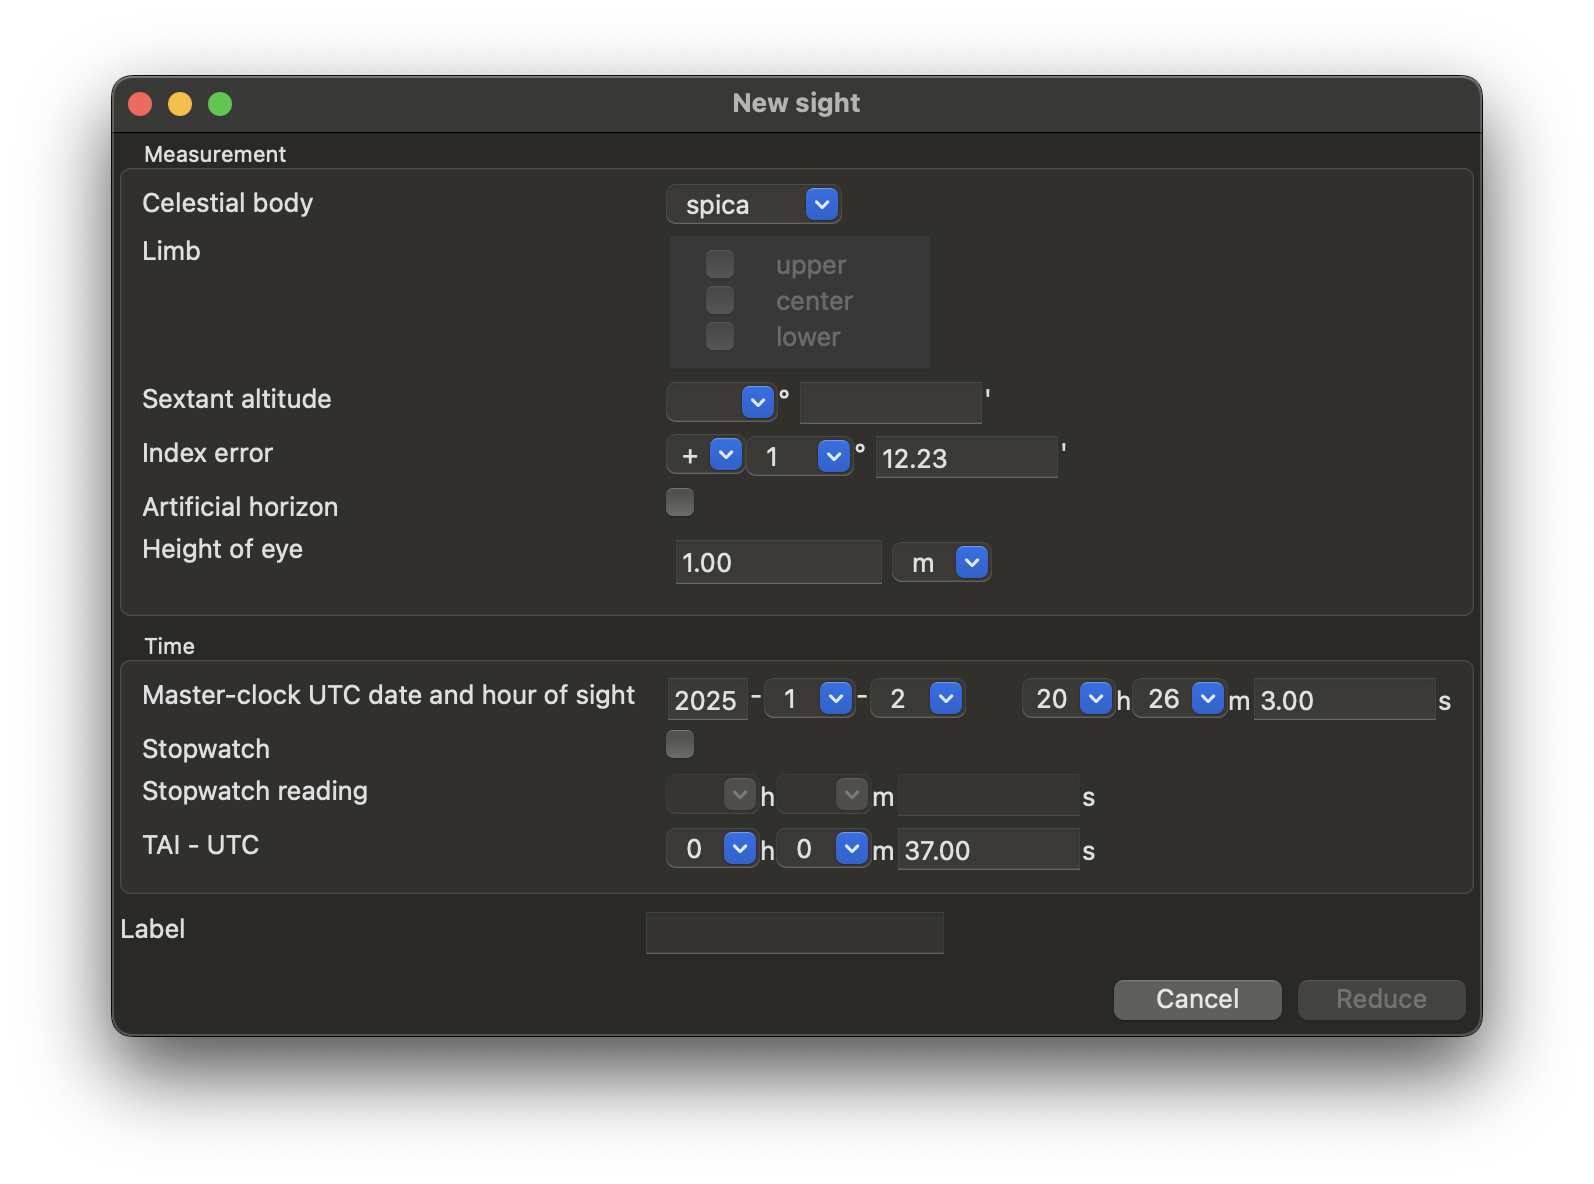
\includegraphics[width=0.9\textwidth]{figures/sight-frame.png}
  \caption{
    \label{fig-sight-frame}
    The sight frame with the entered data from \cref{item-name,item-limb,item-body-height,item-artificial-horizon,item-time,item-label,item-index-error,item-observer-height,item-tai-utc,item-stopwatch,item-tai-utc}. 
  }
  \end{figure}



\printacronyms[pages={display=all,seq/use=false}]
\bibliographystyle{unsrt}
%\addcontentsline{toc}{section}{\refname}
\bibliography{/Users/michelecastellana/Dropbox/my_bibliography/bibliography}


\end{document}
